%\documentclass{article}
\ProvidesClass{configuration/unoesc}
\documentclass[10pt,two column]{configuration/unoesc} 
%Use esse arquivo para incluir novos pacotes

\usepackage[%usado para determinar medidas
top=1.78cm,
bottom=1.78cm,
left=1.65cm,
right=1.65cm,
headsep=0cm,
%showframe
]{geometry}
%\usepackage[justification=centering]{caption}
\usepackage{times}
\usepackage{enumitem}%redefinir espacos itemize
\usepackage{graphicx}
\usepackage{url,hyperref}
\usepackage[utf8]{inputenc}
\usepackage{float}%mais controle para manipular figuras
\usepackage{caption}%manipular legenda da figura e tabela
\usepackage{mathtools}%equacoes
\usepackage[hang,flushmargin]{footmisc} 
\usepackage{xcolor}
\usepackage{wrapfig} %usado para envolver figura com texto
%\usepackage[portuguese]{babel}
\usepackage{fancyhdr}%criacao do cabecalho
\usepackage{etoolbox}
\usepackage[export]{adjustbox}%mais controle para ajustar tamanho da tabela
\usepackage{comment}%ambiente para comentario
\usepackage{relsize} %usado por comandos \mathlarger
\usepackage{lipsum} 

%Referencia bibliografica
\usepackage[
    style=numeric,
    sorting=none,
    maxbibnames=10]{biblatex}
\addbibresource{references.bib}

%Idioma. Use "english" para trabalhos em inglês
\usepackage[english]{babel}
%Ajustes na legenda da figura. Incluindo espacamento apos a legenda
\captionsetup[figure]{labelformat={default},labelsep=period,font=footnotesize, name=\footnotesize{Fig.},justification=centering,singlelinecheck=false,belowskip=0\normalbaselineskip}
%\pagenumbering{gobble}

%Ajustes na legenda da tabela. 
\captionsetup[table]{labelformat={default},labelsep=newline,font={sc,footnotesize},justification=centering,singlelinecheck=false}

%\renewcommand{\headrulewidth}{0pt}

\makeatletter
\newcommand{\linebreakand}{%
  \baselineskip 
  \end{@IEEEauthorhalign}
  \hfill\mbox{}\par
  \mbox{}\hfill\begin{@IEEEauthorhalign}
}
\makeatother


%considerando babel = english
\addto\captionsenglish{
  \renewcommand{\tablename}{TABLE}
}
\usepackage[utf8]{inputenc}
\graphicspath{ {./images/} }
\setlength{\parindent}{0pt}
\usepackage[font=small,labelfont=bf]{caption}
\usepackage{caption}
%\usepackage{subcaption}
\usepackage{subfigure}
%\usepackage[a4paper,top=2cm,bottom=2.5cm,left=2.5cm,right=2.5cm,marginparwidth=1.75cm]{geometry}conference,

\addbibresource{references.bib}

\title{Generation of surface for producing image using caustics}
\author{L.Jiang, Z.Jiang}

\begin{document}

\maketitle
\begin{abstract}
    A continuous surface which generates a given gray-scale image when illuminated by parallel light is computed via caustics and manufactured. The test image and the lens surface were first divided to $N \times N$ grid, where $N$ is determined by the resolution of the test image in pixels ($N=500$ in the first trial). The lens cells were morphed with gradient descend such that each cell (i,j) has area proportional to the brightness of image pixel (i,j). The height-map of the lens surface was then found by applying Snell's law and small angle approximation. Morphing the grid and finding height-map both rely on solving Poisson's equation in Python. A simulation was built to test the output surface, and test images were mostly reproduced at $N=1000$. The surface is then manufactured using acrylic by CNC mill, and tested under parallel light.
\end{abstract}

\section{Introduction}
A given gray-scale image can be produced by reflection or refraction of light rays through curved surfaces or objects. Some methods had been used to obtain such surfaces in computing graphics, for example, reflectance field\cite{reflectancefield}, refractive steganography\cite{refractive}, subsurface scattering\cite{subsurface}, and holography\cite{holography}.\\

Caustics provides satisfactory illumination effect among these methods, with the setup shown in figure \ref{fig:1}. The shape of the transparent material, or specifically the refractive surface, needs to calculated such that it produces the expected caustic image under parallel and normal incident light. Methods proposed by Finckh et al.\cite{finckh}, Papas et al.\cite{papas} and Yue et al\cite{yue}. are restricted by either complexity of patterns or continuity of surfaces. However, Yue et al.\cite{yue2014poisson} suggests a different approach using Poisson's equation, which yields continuous surfaces and highly reproduced patterns. Matt Ferraro\cite{mattwebsite} simplified the above method using Julia without significant loss of outcome image quality. Our aim is to reproduce this result using Python.

\begin{figure}[h!]
\centering
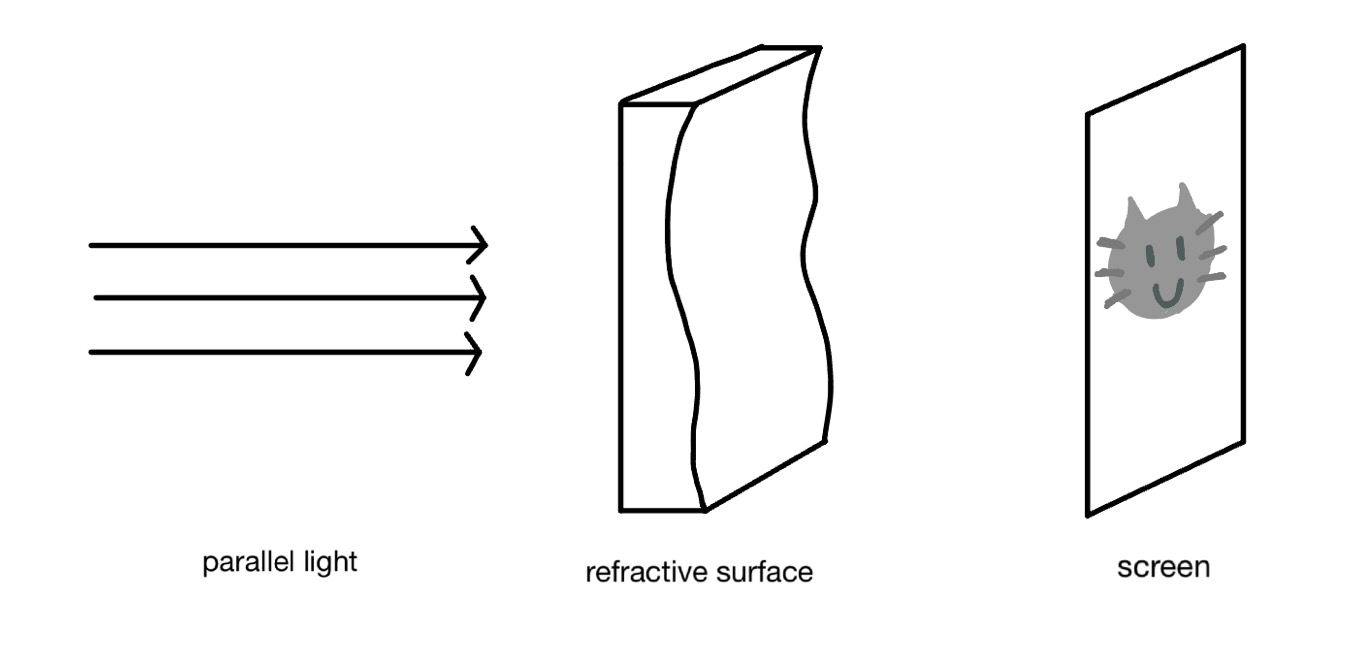
\includegraphics[width=1.0\linewidth]{figures/figure1.jpg} 
\caption{Illustration of display system. Parallel light from either sun or projector, perpendicularly incident on a transparent refractive surface, results in caustic image on the projection screen.}
\label{fig:1}
\end{figure}

\section{Method}
The method described by Yue et al.\cite{yue2014poisson} consists of two steps. First, the corresponding relationship between incident light and the resultant image is determined. After that, the refractive surface is computed through finding its height-map.\\

\subsection{Morphing lens grid}

As demonstrated in Figure 2, for a sample image with $N \times N$ pixels, each pixel is assigned an index $(i,j)$, which does not change over the course of calculations. Since pixels have the same size, the $(u,v)$ coordinate system is essentially a uniform square grid.\\

Next, the refractive surface is also divided into $N \times N$ grids. The index of a particular cell is determined by the index of point on its top left corner, as shown in figure \ref{fig:2}. As such, image pixel $(i,j)$ corresponds to lens cell $(i,j)$. Initially, the grids on refractive plane with coordinates $(x,y)$ will also forms a uniform mesh, but this will change as individual points moves through morphing. Consequentially, the area of lens cell (i,j) can be morphed to be proportional to the light intensity of pixel (i,j) on the image.\\

Mathematically, this process can be thought as a mapping of the $(u,v)$ coordinate system on the image to the $(x,y)$ coordinate system on the refractive surface.\\ 

\begin{figure}[h!]
\centering
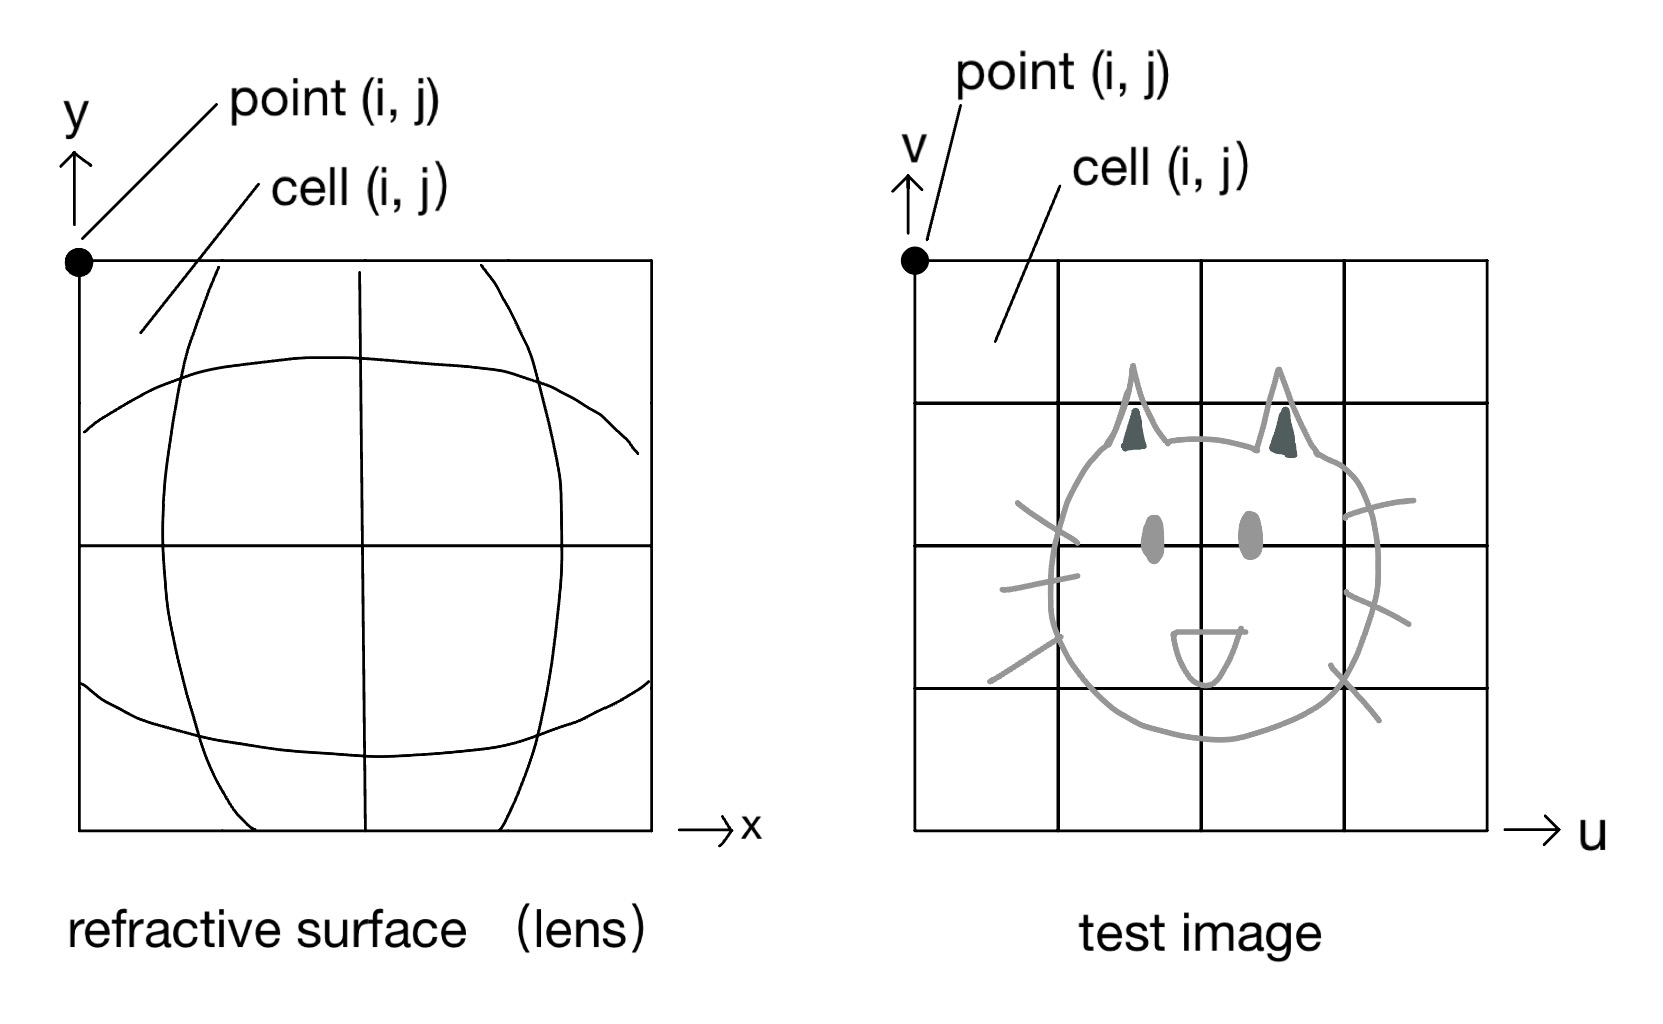
\includegraphics[width=1.0\linewidth]{figures/figure2.jpg} 
    \caption{Corresponding relationship of cells and positions. Each cell $(i,j)$ on the $(u,v)$ plane of the test image corresponds to a cell $(i,j)$ on the $(x,y)$ plane of the refractive surface.}
\label{fig:2}
\end{figure}

Here, an assumption is made such that all light incident on lens cell $(i,j)$ is refracted to pixel $(i,j)$, so no light is lost. Thus, the following must be true,
\begin{equation}
    \frac{A(i,j)}{\Sigma A} = \frac{b(i,j)}{\Sigma b}
\end{equation}
where A(i,j) is the area of cell (i,j) on lens, and b(i,j) indicates the brightness or light intensity of pixel (i,j) on image. Since the refractive surface is divided equally at the beginning, so the cells need to expand or shrink. A scalar field L is used to determine how much the cells are different from the expected value.
\begin{equation}
    L = \frac{b(i,j)}{\Sigma b} -\frac{A(i,j)}{\Sigma A}
\end{equation}
If $L(i,j)>0$ at a point $p(x,y)$, it means the cell is too small and needs to expand. The magnitude of scalar field $L$ is expected to decrease through mapping, so the points can be updated as $\frac{d\vec p}{dt}=-\nabla L$, where $\nabla L$ is the gradient of L (a vector field points to increasing direction) and t is a virtual time defined to represents computational process. However, L is not a continuous scalar field, so $\nabla L$ is a discontinuous vector field, which performs poorly in computation. Therefore, this method is not used.\\

Inspired by computational fluid dynamics, instead of finding gradient of L, a concept 'pressure field' is applied. The analogy between cells with positive and negative L with source and sink with high and low pressure allows us to regard the mapping process as relaxation of source and sink, where flux flows form high pressure to low pressure. Therefore, with a pressure field $\phi$, we have:
\begin{equation}
    \frac{d\vec p}{dt} = \nabla \phi
\end{equation}
The concept, divergence, is also used to connect the pressure field $\phi$ to the scalar field L. Divergence of a vector field is a scalar field, which represents the outward flux from an infinitesimal volume around a given point. For example, consider the case heating air. Velocity of air molecules generates a vector field, when air is heated in a region, air molecules expands in all directions, so the divergence of the velocity vector field is positive. Similarly, in our case, cells with positive L expands and with negative L shrinks, the greater L is, the more it needs to expand. Therefore, we obtain the following equation:
\begin{equation}
    \nabla^{2} \phi = L
\end{equation}
Solving this Poisson's equation gives a continuous and well behaved scalar field $\phi$. Positions p(x,y) of points (i,j) is updated repeatedly by computing the difference L, solving equation(4) and updating according to equation(3).\\

A square mesh is used to compute L. Gauss-Seidel method is applied to solve Poisson's equations, with Neumann boundary condition and over-relaxation parameter $\sigma=1.94$. The vertices of the square mesh is updated using equation $\vec p(t_{n+1})=\vec p(t_n)+ \Delta t\nabla \phi$, where n indicates the $n^{th}$ computation step. For the points on the edge, their movement is restricted within the side they lie on. A suitable $\Delta t$ needs to be found for each iteration so that vertices do not surpass their neighbours. To achieve this, the program iterates through all points, finding the limiting case of $dt$ such that the closest two points would be coincidental, and returns half of $dt$ to be $\Delta t$ \cite{yue2014poisson}.

\subsection{Finding Heightmap}
After morphing the grids, the z coordinates, or a scalar field $z=h(x,y)$ is computed. A normal vector $\vec N$ to the refractive surface can be represented by taking gradient of the surface $z=h(x,y)$, which is:
\begin{equation}
    \vec N = (\frac{dh}{dx},\frac{dh}{dy},-1)
\end{equation}
where the z component is normalized to be 1. Define a vector $\MakeUppercase N_{xy}$ contains only x and y component, we have:
\begin{equation}
    \vec N_{xy} = \nabla h
\end{equation}
The two component of N can be calculate using Snell's law and small angle approximation\ref{fig:3},
\begin{equation}
    N_{x} = tan \frac{tan^{-1}(\frac{u-x}{d})}{(n_1-n_2)}
\end{equation}
\begin{equation} 
    N_{y} = tan \frac{tan^{-1}(\frac{v-y}{d})}{(n_1-n_2)}
\end{equation}
where $n_1 = 1.49$ and $n_2 = 1$ are the refractive index of acrylic and air. Therefore, a second Poisson's equation is obtained by taking divergence of both sides, 
\begin{equation}
    \nabla^2 h = \div{{\vec N_{xy}}}
\end{equation}

\begin{figure}[t!]
\centering
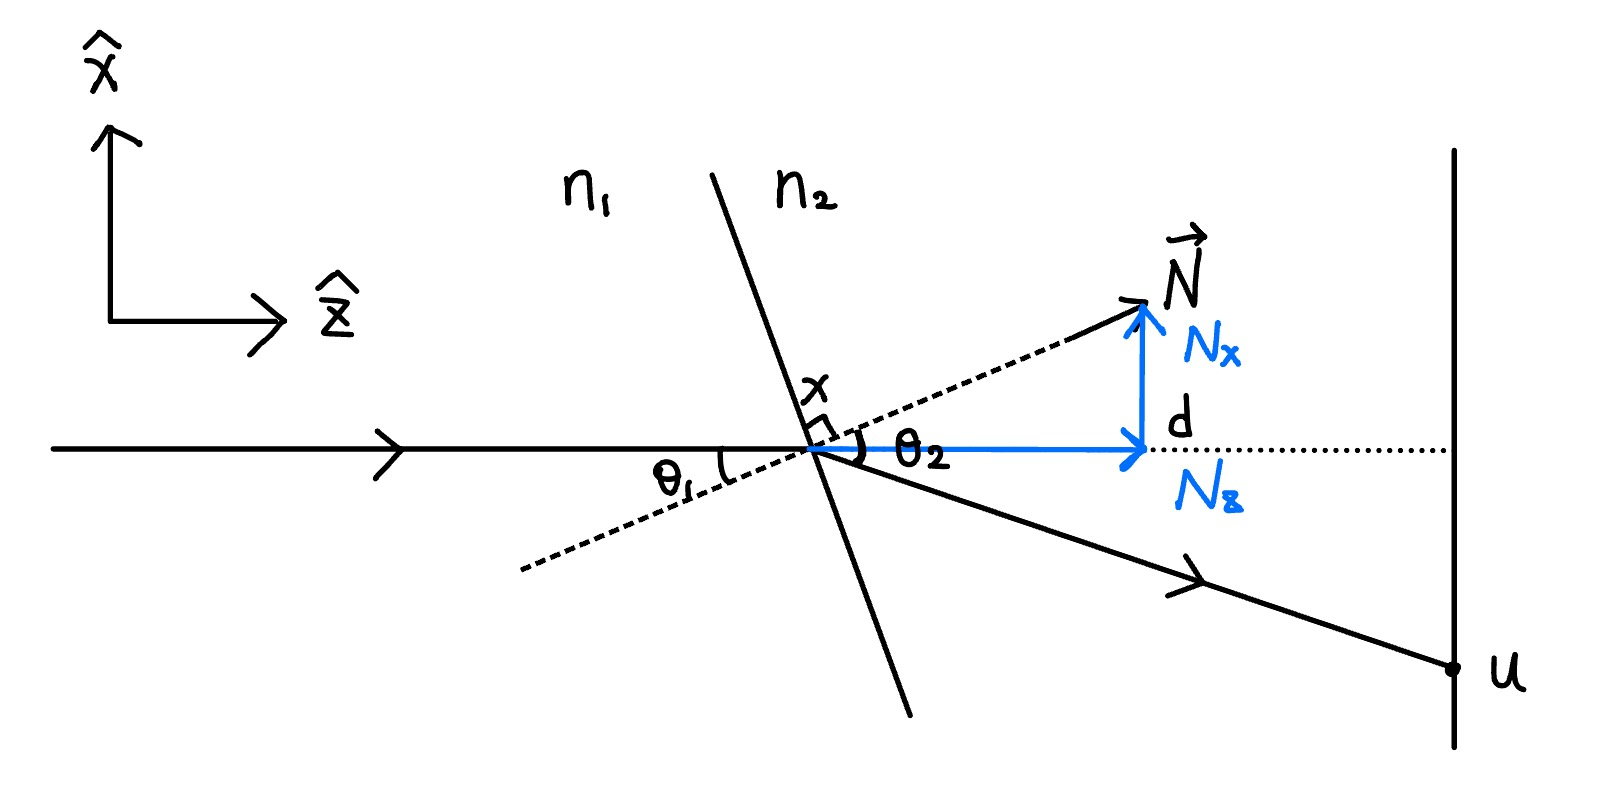
\includegraphics[width=1.0\linewidth]{figures/figure3.jpg} 
\caption{Refractive in x direction. Light incident at coordinate x on the lens is refracted onto coordinate u on the screen. Using Snell's law, $\frac{sin(\theta _1)}{sin(\theta _2)}=\frac{n_2}{n_1}$, and small angle approximation, $\frac{\theta_1}{\theta_2}=\frac{n_2}{n_1}$, equation links $\theta_1$ and $\theta_2$ is obtained. By geometry, assuming d is much greater than x and u, $\theta_1 = \theta_2 - tan^{-1}(\frac{x-u}{d})$. Normalizing $\MakeUppercase N_{z}$ gives $\MakeUppercase N_{x} = tan(\theta_1)$.}
\label{fig:3}
\end{figure}

Initially, the refractive surface is set as a plane, so the distance $d(x,y)$ between the refractive surface and the projection screen is uniform. Components of $\vec N$ in $x$ and $y$ direction and gradient of vector field $ \vec N_{xy}$ are then computed using equation (7), (8). A heightmap is found by solving equation (9), so that an updated scalar field $d(x,y)$ can be calculated. These processes are repeated until convergence. The mesh is then organized into .stl format for manufacture.\\

\subsection{Computational Simulation}
The refractive surface obtained by combining results form the above two steps is tested using a simulation program.\\

Each cell (i, j) is split into two triangles. For each triangle, the normal vector is obtained using the plane defined by vertices. Incident light in the direction of (0, 0, 1) is divided into parallel and orthogonal components with respect to the normal vector of the cell. According to Snell's law, the output parallel component is scaled by factor of $\frac{n_1}{n_2}$ and the output perpendicular component remains unchanged. Thus, the direction of light (output vector) after refractive is found. For simplicity, all light that lands on the triangle is assumed to be transmitted through the center. Under this assumption, the output vector is scaled to find landing point on screen. If the landing point is within a grid, the area of triangle is added to corresponding point (u,v). If the landing point is outside the grid, the incident is recorded, and the light is considered lost. These process are shown in Figure 4\ref{fig:4}.\\

\begin{figure}[h!]
\centering
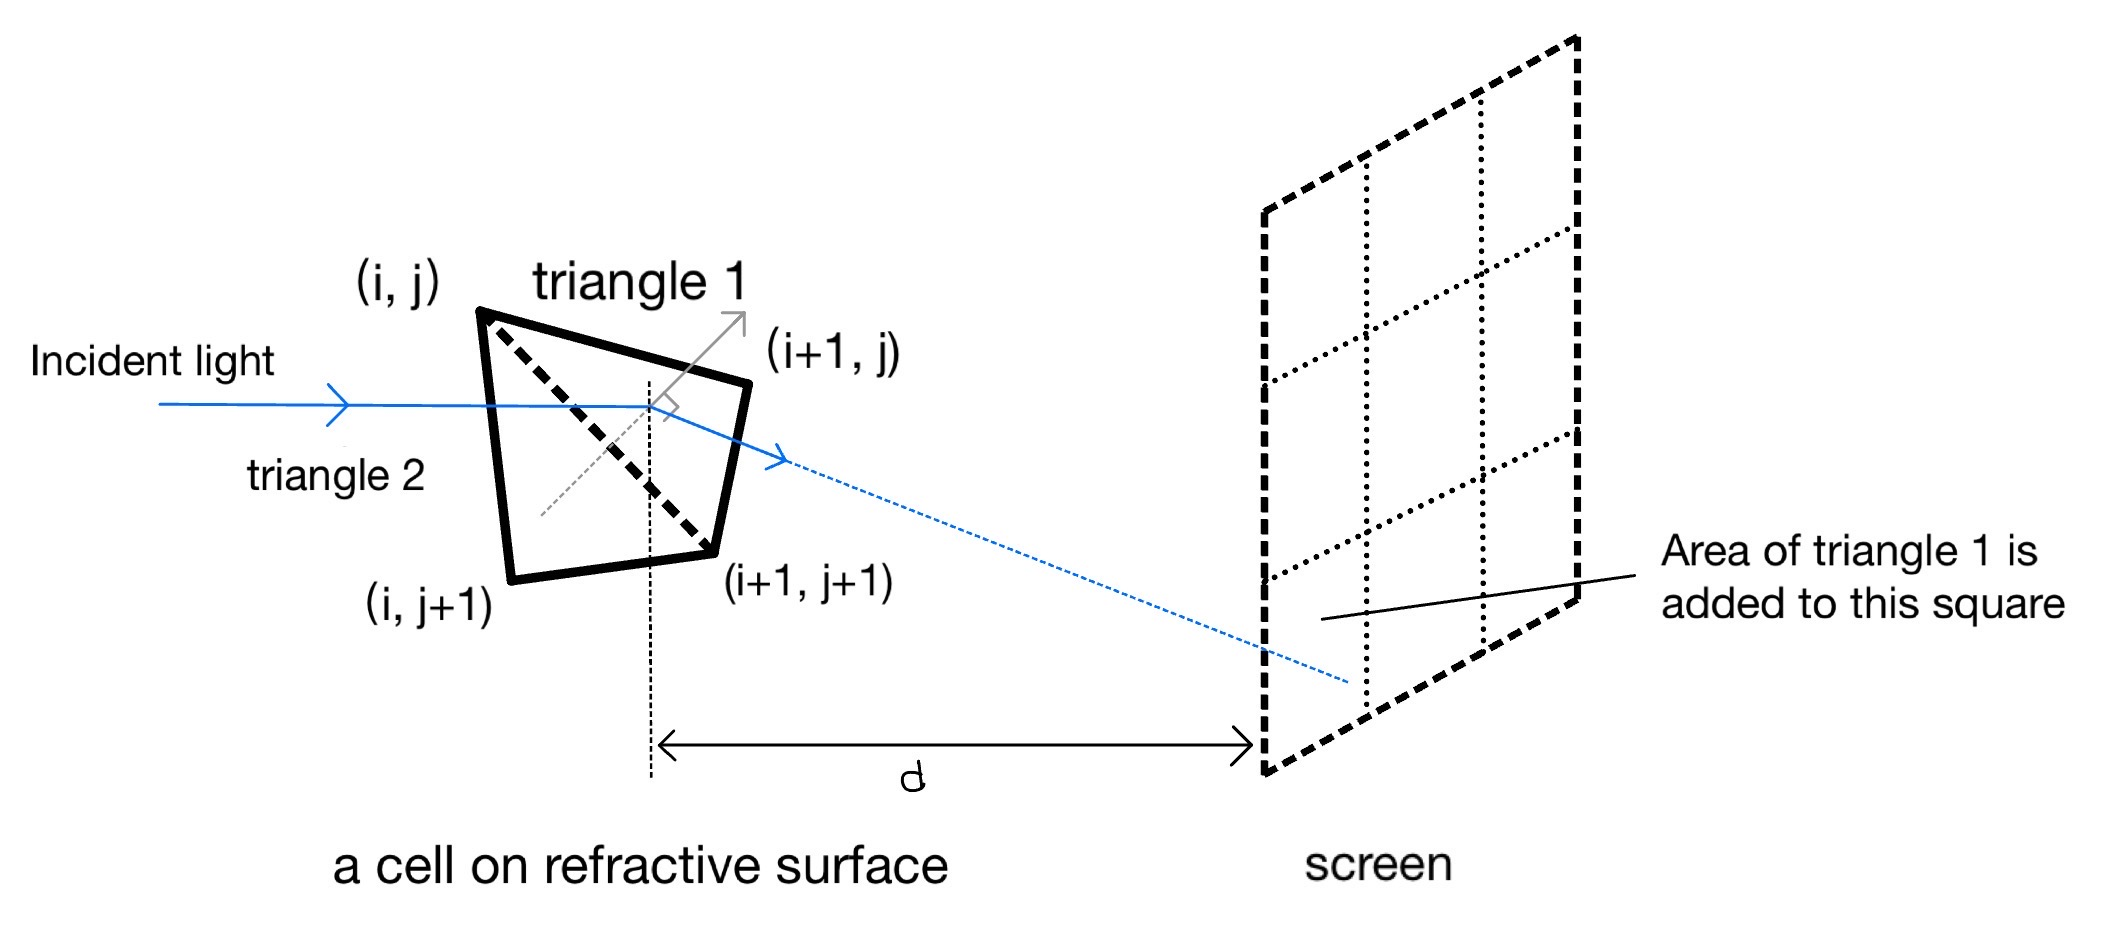
\includegraphics[width=1.0\linewidth]{figures/simulation.jpg} 
\caption{Simulation of refraction for one piece of triangular surface.}
\label{fig:4}
\end{figure}

After repeating the process for all triangles, the average of all points is scaled to 128, or half the maximum brightness in grey-scale. The result is saved as a .png file.\\

\section{Results}

\subsection{Simulation Result}

Simulation results are shown in figure 5, where the test images are put on the left and the results on the right. Some accuracy is lost at small details, and the outline of objects tend to get distorted in the process. Nevertheless, the images are highly reproduced. \\

\begin{figure}[h!]
\subfigure{
\includegraphics[width=0.23\textwidth]{figures/figure511.png}}
\hspace{0.01\textwidth}
\subfigure{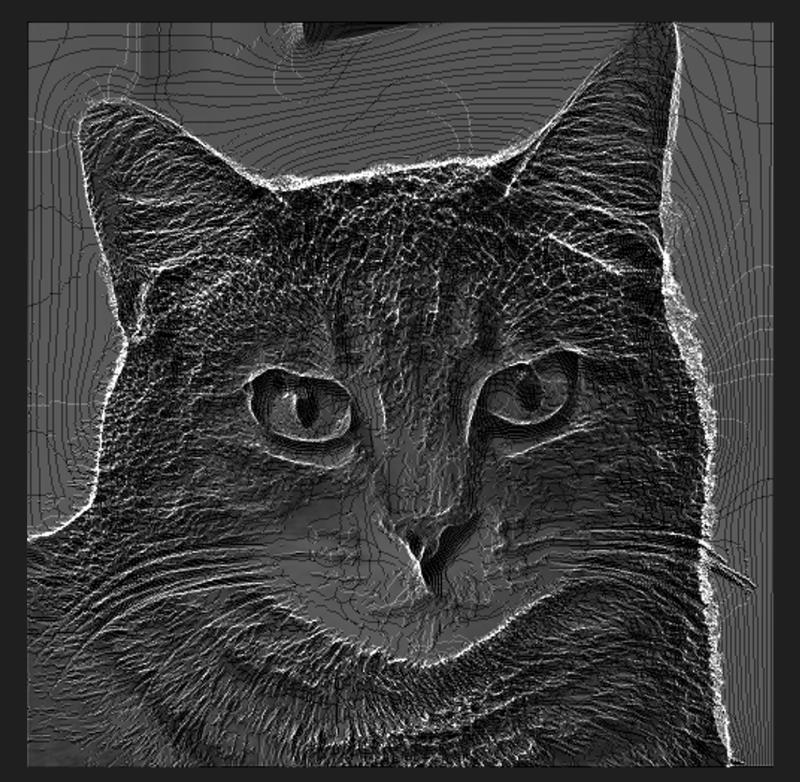
\includegraphics[width=0.23\textwidth]{figures/figure512.jpg}}
\hspace{0.01\textwidth}
\subfigure{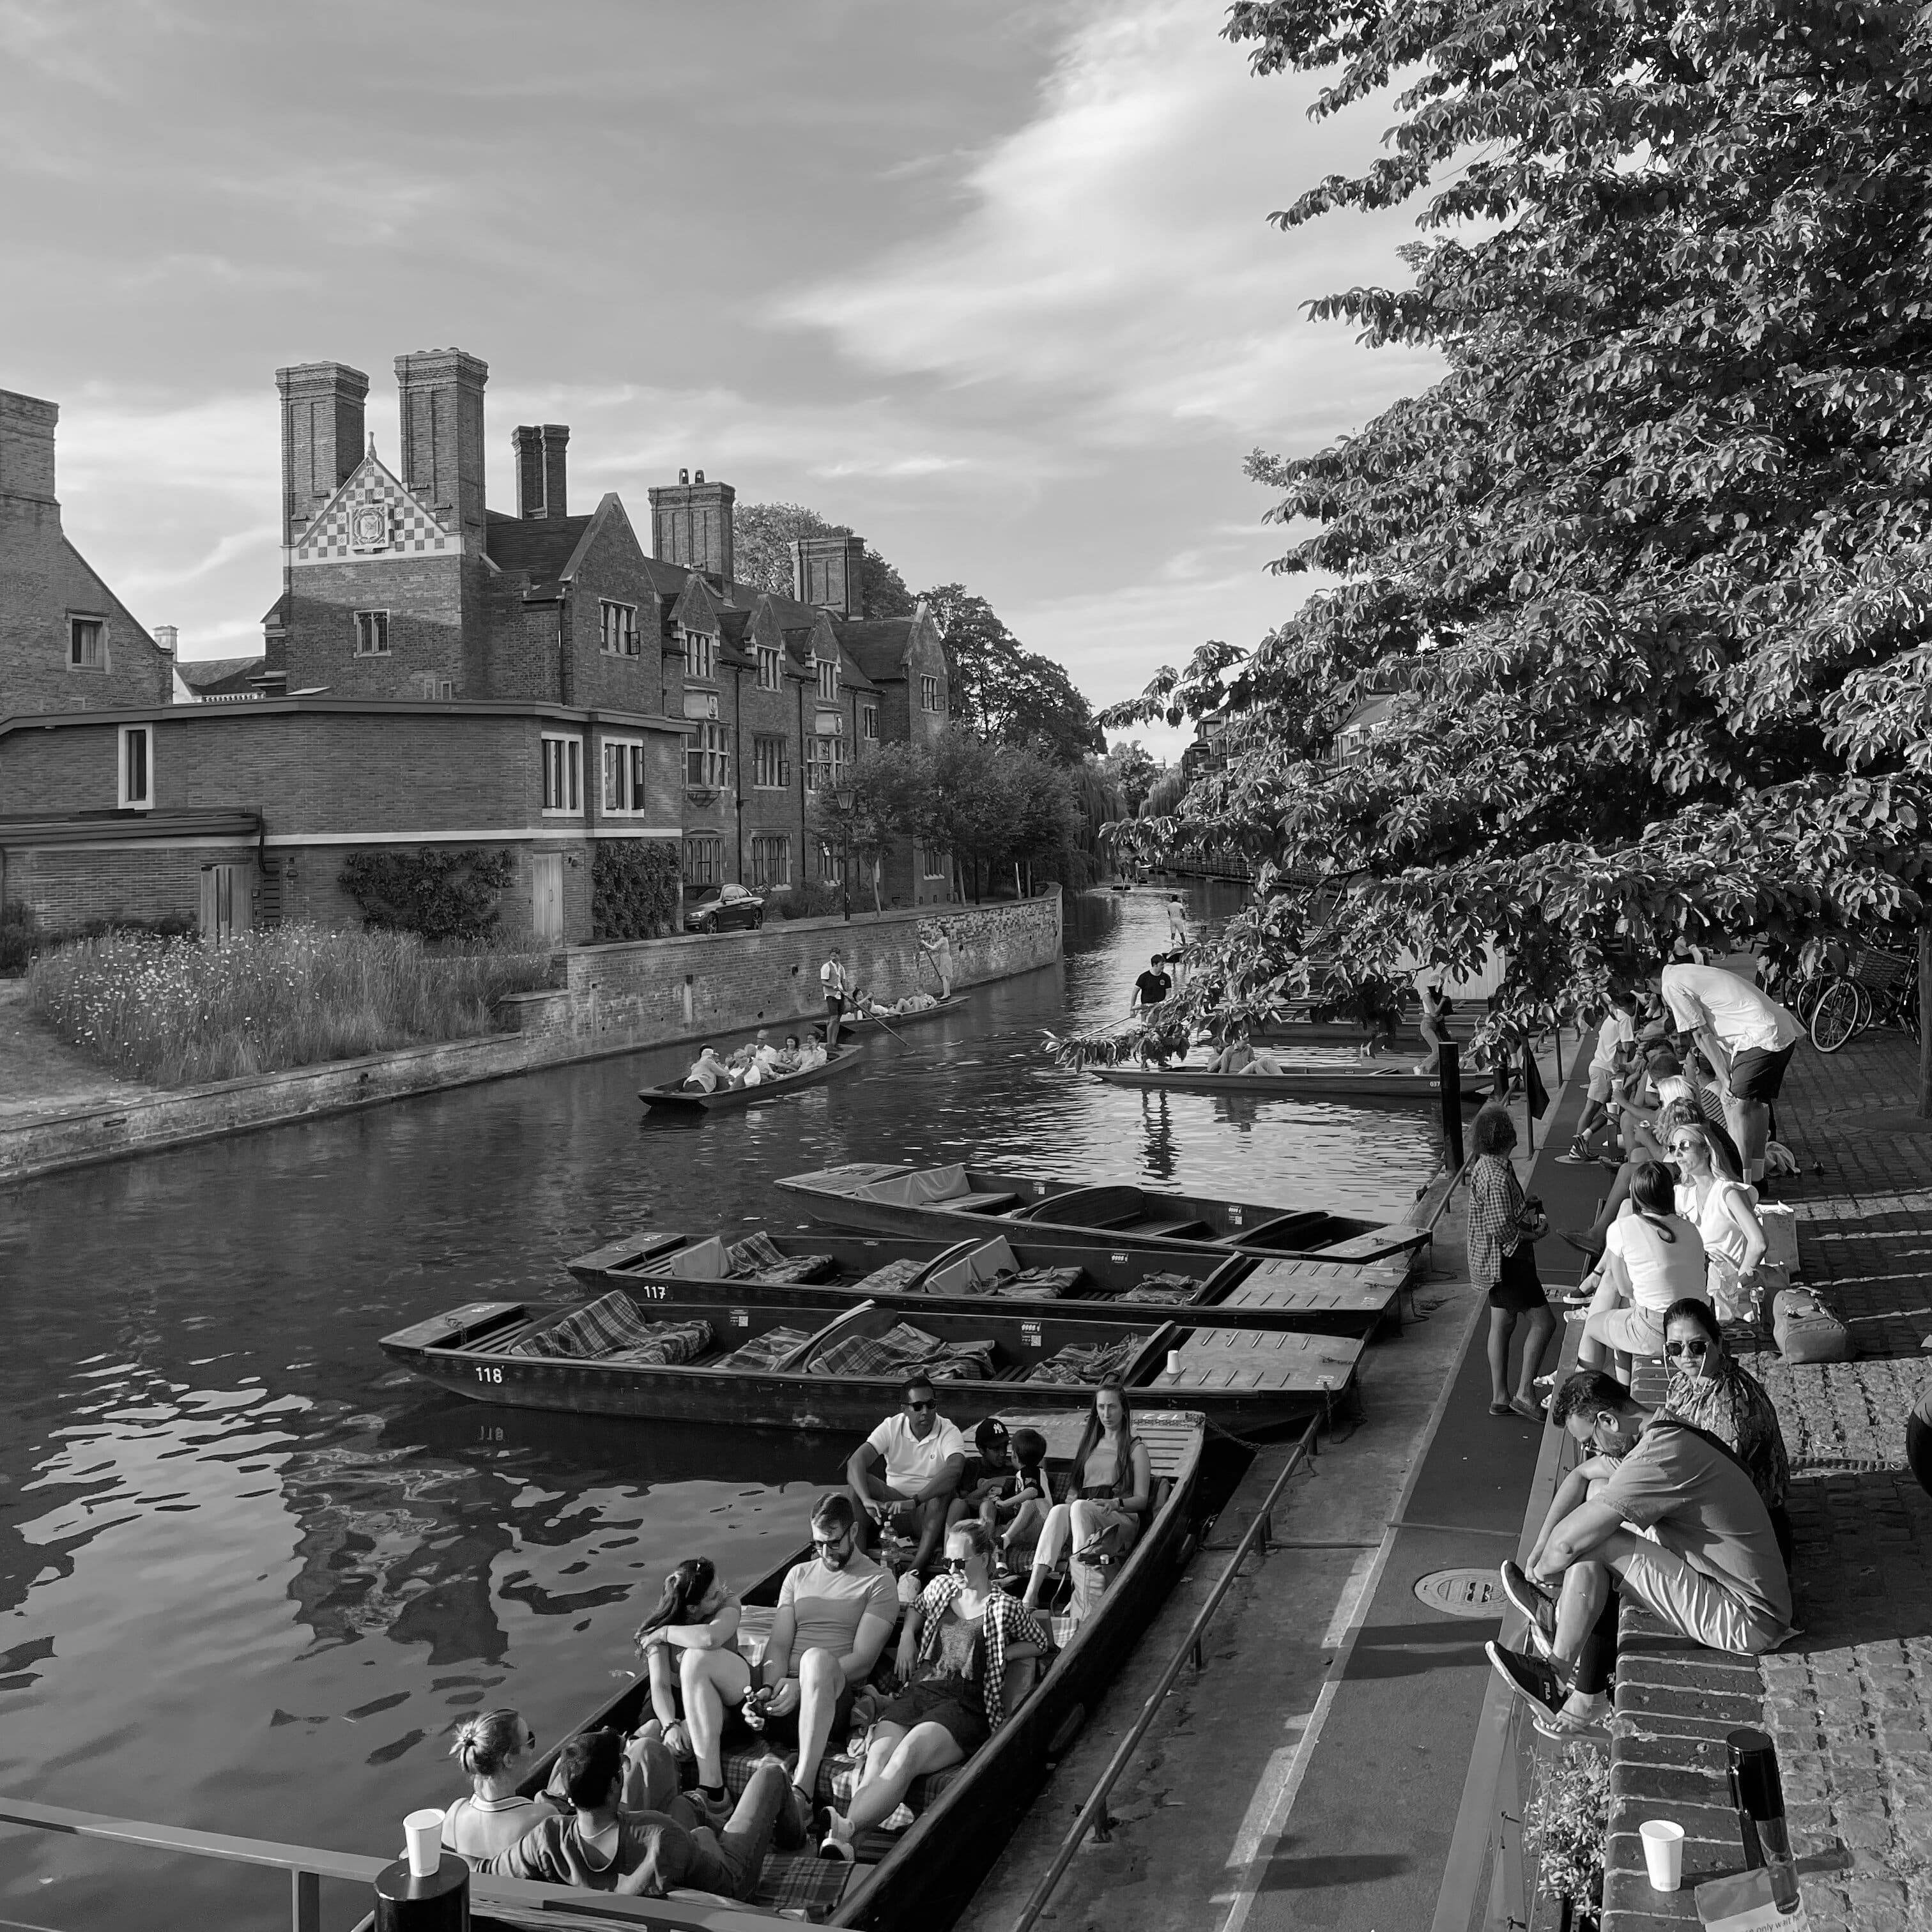
\includegraphics[width=0.23\textwidth]{figures/figure521.jpg}}
\hspace{0.01\textwidth}
\subfigure{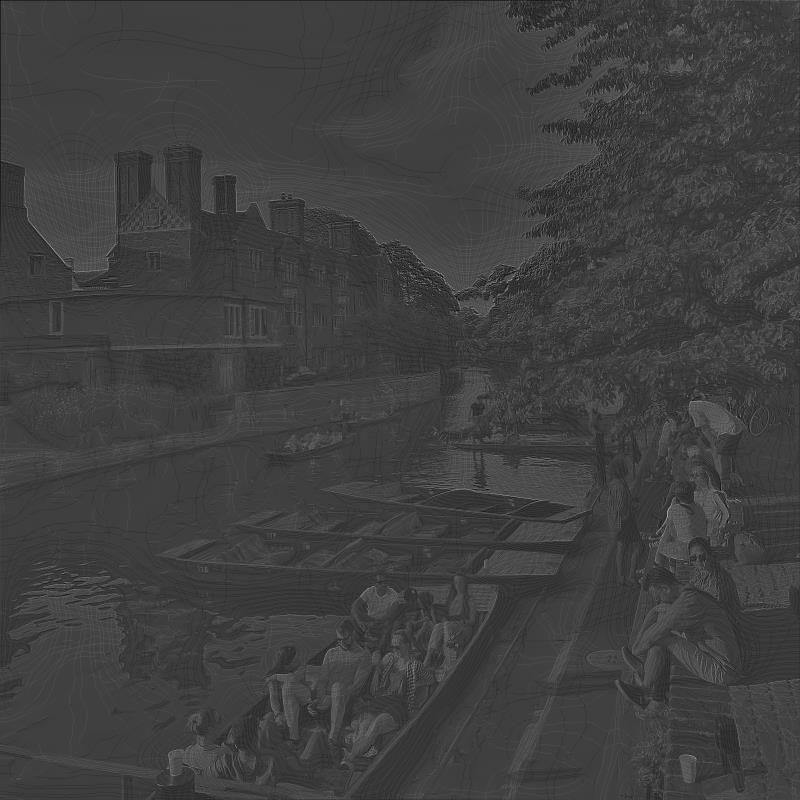
\includegraphics[width=0.23\textwidth]{figures/figure522.jpg}}
\hspace{0.01\textwidth}
\subfigure{
\includegraphics[width=0.23\textwidth]{figures/figure531.png}}
\hspace{0.02\textwidth}
\subfigure{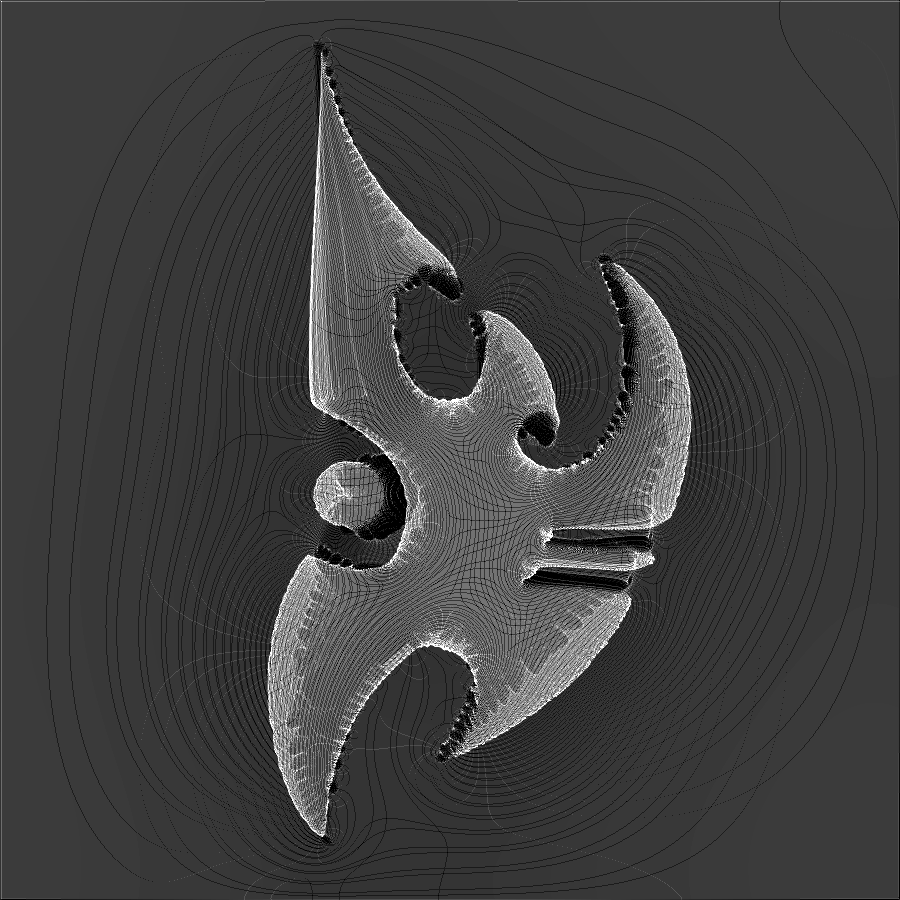
\includegraphics[width=0.23\textwidth]{figures/figure532.png}}
\caption{Input images compared with simulated outputs. Resolutions are 500, 3000 and 900 separately.}
\label{fig:5}
\end{figure}

\subsection{Manufactured Result}
The acrylic lens are manufactured using a Roland MDX-40A Benchtop CNC Mill. Multiple setups were attempted with mixed results. The setup that yielded the smoothest surface was using R3 ball nose as both roughing and finishing tool. The resulting parts are then wet sanded with 400, 600, 800, 1000, 1200, and 1500 grit sandpapers. The parts are then washed and dried, before the fine and finish Tamiya polishing compounds are applied.\\ % Figure of result.

\section{Discussion}

\subsection{Computational process}

To morph the grids, a $(N+1)\times(N+1)$ vector field is required (as there is $(N+1) \times (N+1)$ points in total), however, the $N \times N$ scalar field $\Phi$ is not sufficient to generate such a vector field.  For the purpose of obtaining sufficient information, the scalar field is mirrored with respect to all four of its edges, turning the scalar field to $3N \times 3N$. Only the $(N+2) \times (N+2)$ data points in the center is used. A demonstration of the mirroring step for a $2 \times 2$ field is shown in Figure 5\ref{fig:6}. This method simplifies the program and also automatically applies Neunmann boundary conditions. \\

\begin{figure}[h!]
\centering
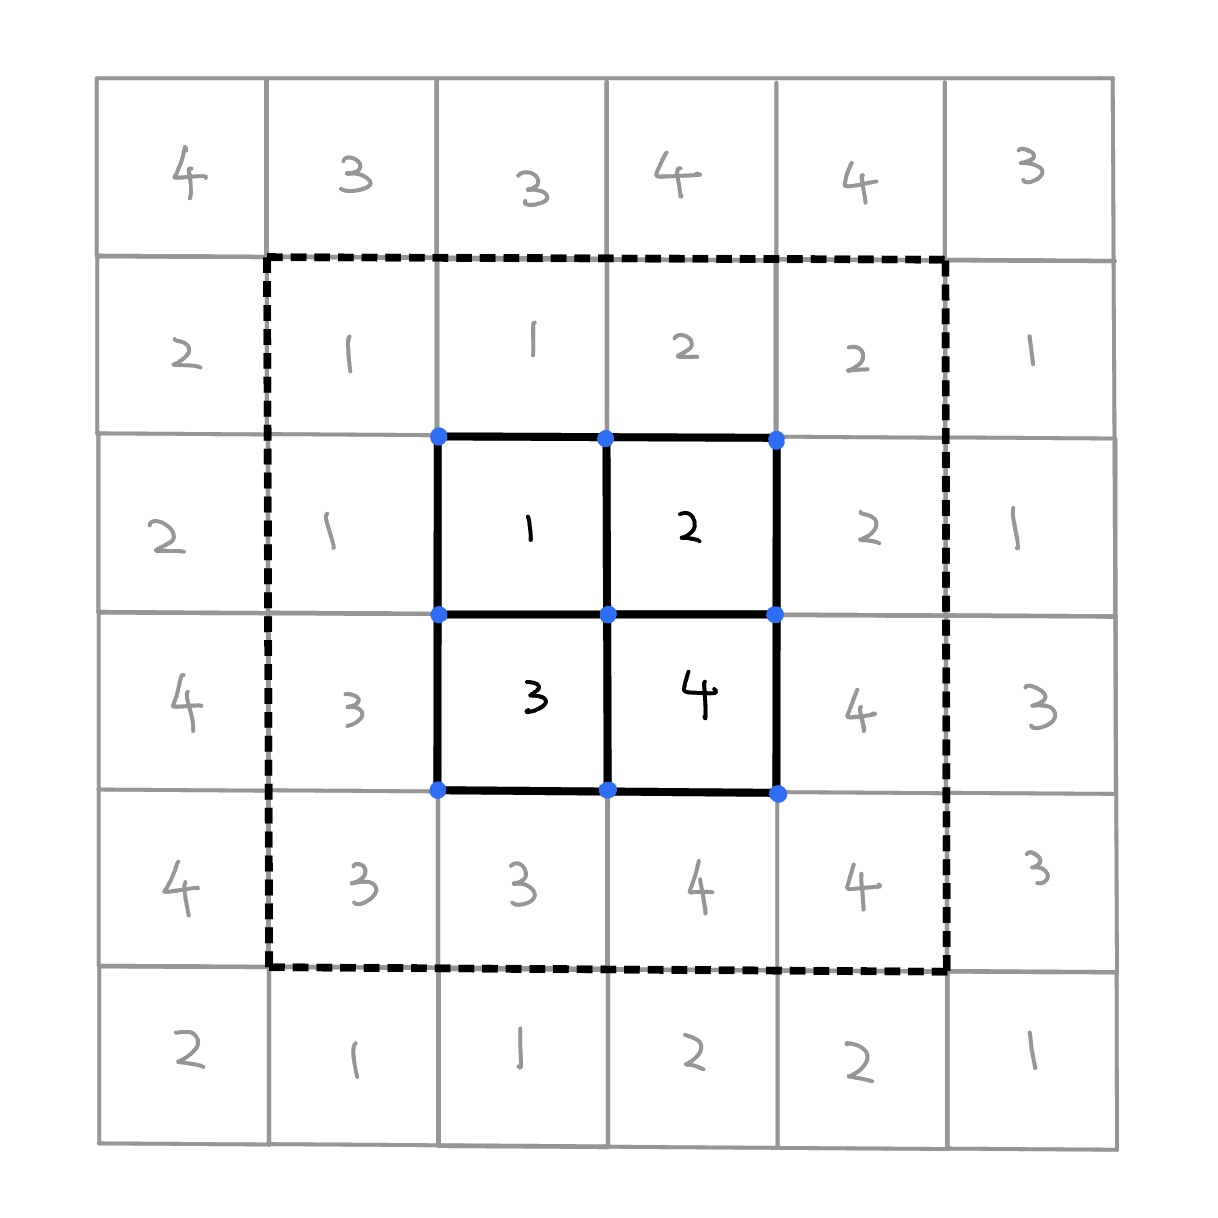
\includegraphics[width=0.7\linewidth]{figures/mirror.jpg} 
\caption{Mirror for a $2 \times 2$ scalar field for demonstration. The $4 \times 4$ data in the dotted square is used to obtain $3 \times 3$ vectors (blue points).}
\label{fig:6}
\end{figure}

The computational process is extremely time consuming to use on pictures with high resolution since the algorithm has a $O(n^2)$ complexity, it takes about 30 minutes for $500 \times 500$ and about 5 hours for $3000 \times 3000$. Therefore, a suitable resolution need to be chosen for each test image, such that it takes the program reasonable amount of time to finish calculation and generates a relative high-quality output. Most images were initially tested with a version that has reduced resolution ($300 \times 300$ or less). Numba was used to speed up calculations for high-resolution images.

\subsection{Errors and limitations}

The most efficient way to simulate a 3-D surface is triangle mesh, while square mesh is used in the program, which may leads to decrease of accuracy. In addition, when calculating height-map, interference effect is ignored. This effect is hard to avoid in reality, which limits the output image quality. Moreover, the fact that light passes through the entirety of the cells and may land on multiple pixels is not taken into account in the simulation program, resulting in great amount of error. However, these error can be diminished using high resolution. \\

A focus distance is assumed in advance when solving the height-map, but the whole refractive surface moves further from the screen during iteration process, resulting in difficulty to determine the exact output surface focus distance. Also, this method limit the distance d between refractive surface and screen to a range, output images quality drops significantly if d is out of range.\\

However, despite the resulting image being similar to the input, the simulation program suggests that less than 2\% of the light actually land at where they are expected to land. Such result suggests that the accuracy of the height-map is less than expected. \\

\subsection{Manufacturing}

Initially, a 1mm square nose is used for roughing, and a engraving tool with 0.02mm tip is used for finishing. This yielded a rough and nontransparent surface. Later approaches used R3 ball noses for both roughing and finishing with mixed results. By far, the smoothest surface is achieved using a R3 ball nose as roughing tool with 0.37mm cut-in stepping and 0.05mm path interval, and a R2 ball nose as finishing tool with 0.37mm cut-in stepping and 0.20mm path interval with 0.37mm cut-in stepping and 0.05mm path interval.\\

\begin{figure}[h!]
\centering
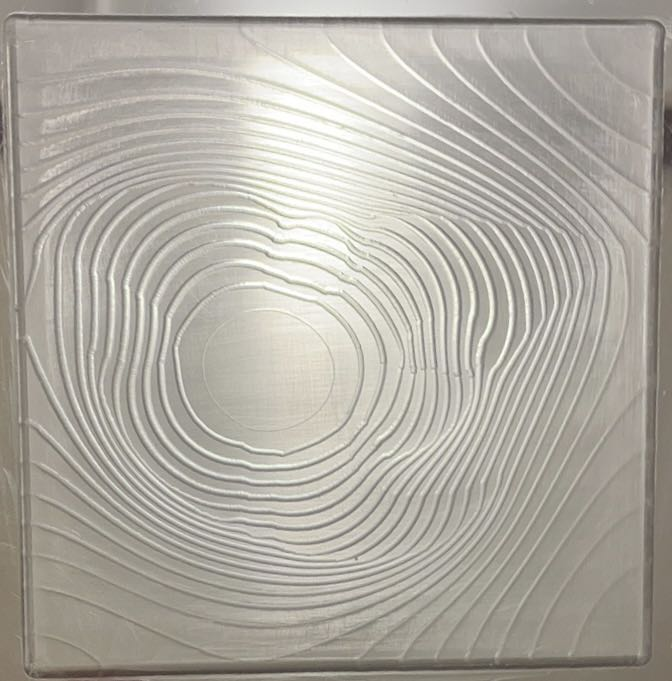
\includegraphics[width=0.5\linewidth]{figures/surface.jpg} 
\caption{The surface of the manufactured acrylic lens}
\label{fig:7}
\end{figure}

\begin{figure}[h!]
\subfigure{
\includegraphics[width=0.23\textwidth]{figures/figure531.png}}
\hspace{0.01\textwidth}
\subfigure{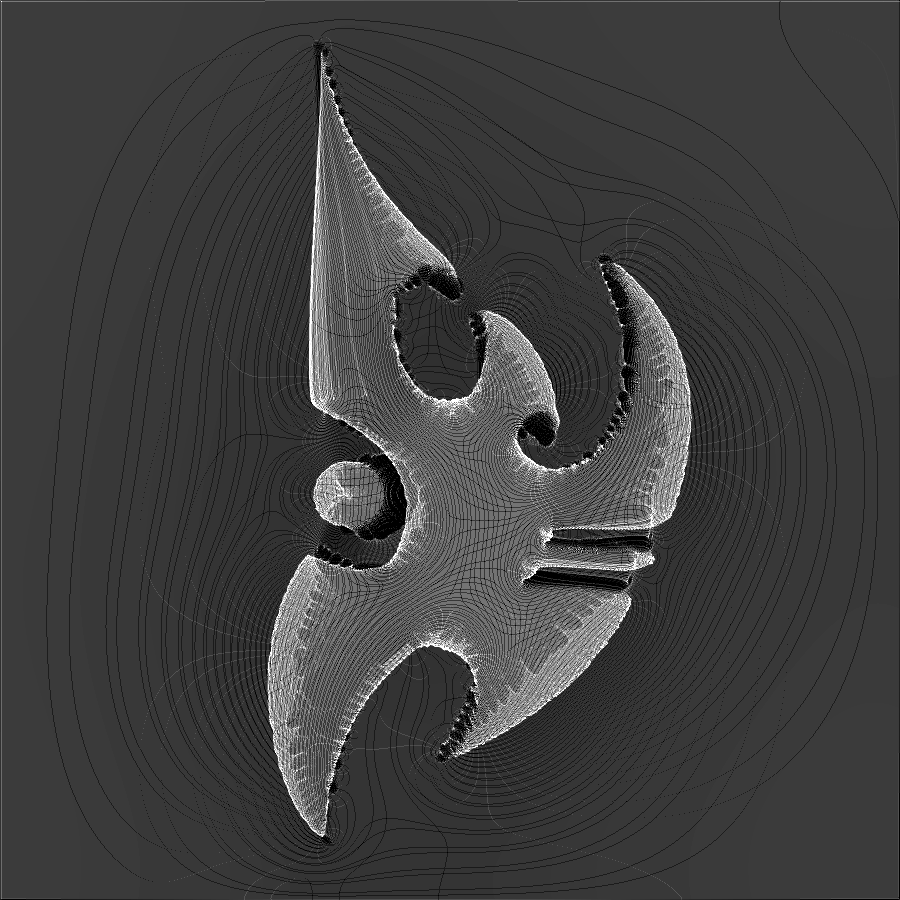
\includegraphics[width=0.23\textwidth]{figures/figure532.png}}
\hspace{0.01\textwidth}
\subfigure{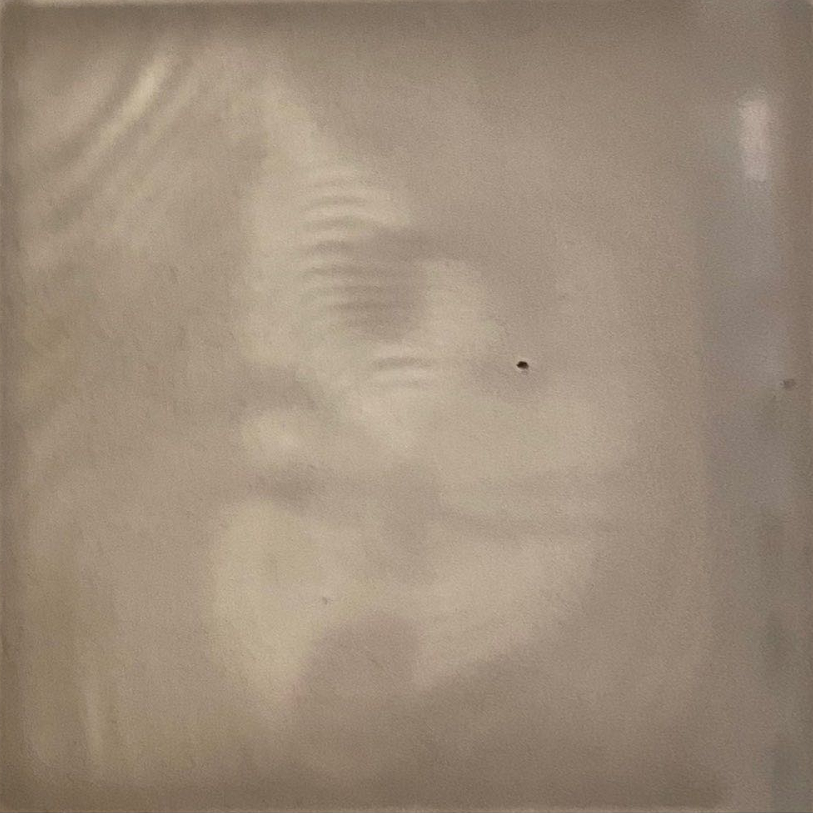
\includegraphics[width=0.23\textwidth]{figures/figure61.png}}
\hspace{0.02\textwidth}
\subfigure{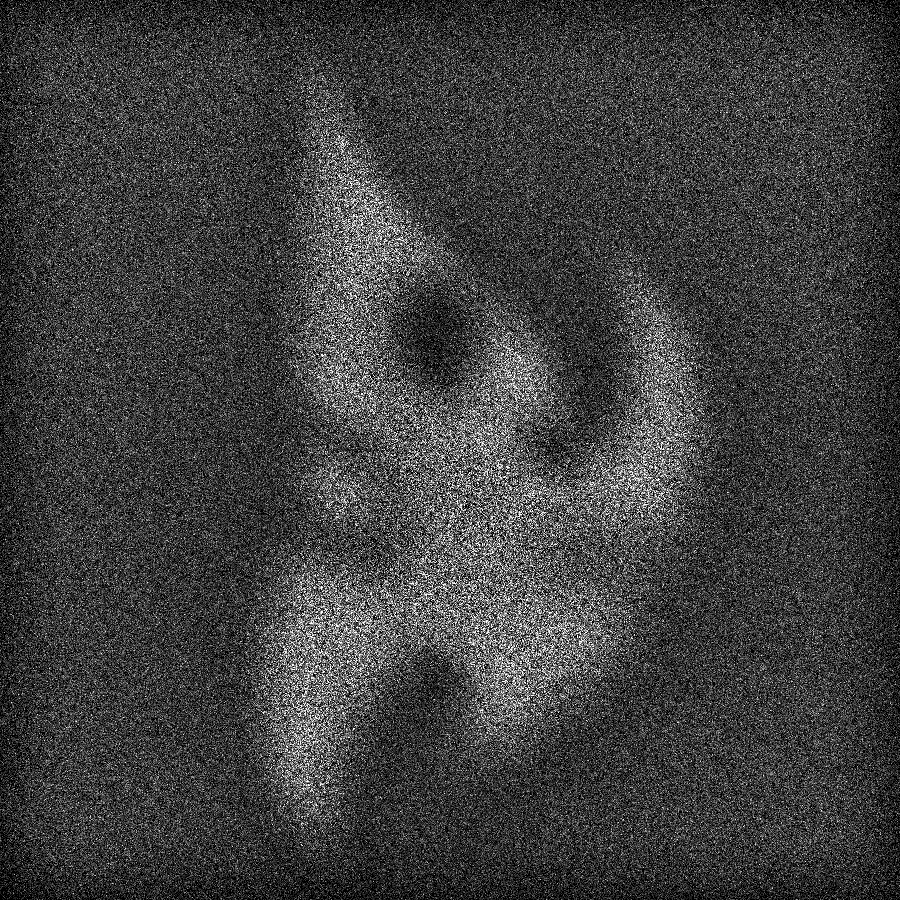
\includegraphics[width=0.23\textwidth]{figures/figure62.png}}
\caption{In order: input image, simulated output with no error, manufactured object output, simulated output with max +/- 0.01mm error}
\label{fig:8}
\end{figure}


The manufactured objects are also severely affected by the contour lines created by the CNC mill, which are impossible to remove them with sandpaper without significantly changing the heightmap. The edges of the contour lines cast shadows on the projection plane and severely affects the quality of the output image. Unfortunately, the Roland MDX-40A CNC does not offer the option to remove the contour lines, only upcut or downcut. With alternate settings, this issue can be partially suppressed, at the cost of some accuracy.\\

The tolerance of CNC milling also limits the performance of the acrylic lens. The standard CNC tolerance is set around +/-0.127 mm. If this is included in the simulation, with every point's z coordinate off by a random number between 0 to 0.01 mm, the resulting output would be a lot closer to the output of the manufactured lens. \\

\section{Conclusion}
In conclusion, shape of a refractive surface, which is able to form a specific caustic image under parallel light, was computed using methods proposed by Matt Ferraro\cite{mattwebsite} and Yue et al\cite{yue2014poisson}. Concepts in computational fluid dynamics are used to morph the image to the surface, then height-map of the surface is calculated. A computational simulation was built to test the code. Simulation results shows that the target image is highly reproduced with high resolution. The refractive surface was then manufactured by CNC machine and tested under lamp light. Even though only simple caustic patterns were able to be reproduced due to technical limitations, the experimental result proves effectiveness of the computational process. For future improvements, methods for solving poisson equation with greater accuracy and speed can be used. In addition, the computational process can be modified to improves edge representation.

\printbibliography

\end{document}



